\documentclass[]{article}
\usepackage{graphicx}
\usepackage{amsmath}		% For generic math symbols
\usepackage{amssymb}		% For mathbb
\usepackage{enumerate}		% For lists indexed by letters
\usepackage{bm}				% For bold symbols
\usepackage{enumitem}		% So we can resume counting problem numbers after
							% interrupting with text

\setlength{\parindent}{0pt}	% Turns off indentation


% Set some useful commands
\newcommand{\half}{\frac{1}{2}}
\newcommand{\R}{\mathbb{R}}
\newcommand{\bbm}{\begin{bmatrix}}
\newcommand{\ebm}{\end{bmatrix}}
\newcommand{\bnm}{\begin{Vmatrix}}
\newcommand{\enm}{\end{Vmatrix}}
\newcommand\norm[1]{\begin{Vmatrix}#1\end{Vmatrix}}
\newcommand\nsum[1]{\| #1 \|_{sum}}

% Place this command after each problem, before solution (examples below)
\newcommand{\solution}{\vskip 0.5cm \textbf{\large Solution:} \\}


\title{AMATH 352: Problem set 1 solutions}
\author{Dave Moore, dmmfix@uw.edu}

\begin{document}

\maketitle

\section*{Column Vectors:}

% The enumerate environment is used for numbered lists. Each time you want to
% add another number to the list, use the \item command
\begin{enumerate}
  
  % First problem
\item Show that for any $\alpha\in\R$ and any $\bm{x},\bm{y}\in\mathbb{R}^m$, $\alpha(\bm{x}+\bm{y}) = \alpha\bm{x} + \alpha\bm{y}$.
  
  \solution
  By definitions (1.2) and (1.3):

  \[
    \begin{split}
       \alpha (\bm{x} + \bm{y}) & =
      \begin{bmatrix}
        \alpha (x_{1} + y_{1}) \\
        \alpha (x_{2} + y_{2}) \\
        \vdots \\
        \alpha (x_{m} + y_{m}) \\
      \end{bmatrix} \\
      &=
      \begin{bmatrix}
        \alpha x_{1}  + \alpha y_{1} \\
        \alpha x_{2}  + \alpha y_{2} \\
        \vdots \\
        \alpha x_{m} + \alpha y_{m}
      \end{bmatrix} \\
      &=
      \begin{bmatrix}
        \alpha x_{1} \\
        \alpha x_{2} \\
        \vdots \\
        \alpha x_{m}
      \end{bmatrix} +
      \begin{bmatrix}
        \alpha y_{1} \\
        \alpha y_{2} \\
        \vdots \\
        \alpha y_{m}
      \end{bmatrix} \\
      &=
      \alpha\bm{x} + \alpha\bm{y}
    \end{split}
  \]  
  
  % Next problem
\item Show that for every vector $\bm{x}\in\mathbb{R}^m,~ 1\bm{x}=\bm{x}$.

  \solution
  By definition (1.3):

  \[
      1 \bm{x} =
      \begin{bmatrix}
        1 x_{1} \\
        1 x_{2} \\
        \vdots \\
        1 x_{m}
      \end{bmatrix} \\
      =
      \begin{bmatrix}
        x_{1} \\
        x_{2} \\
        \vdots \\
        x_{m}
      \end{bmatrix} \\
      = \bm{x}
  \]  

\end{enumerate}


\section*{Norms and inner products:}

\begin{enumerate}[resume]
	
	% Next problem
	\item Determine whether each of the following functions is a norm. Justify your answer, i.e. if you claim it is a norm, show that it satisfies the five criteria discussed in class, and if not, give a concrete example that shows it doesn't satisfy one of the criteria.
	
	% Creating an enumerate environment inside another enumerate environment creates a sub-list
	\begin{enumerate}
		\item $\bm{x}\in\R^3$, $\|\bm{x}\| := \|\bm{x}\|_2-\|\bm{x}\|_1$
		\item $\bm{x}\in\R^3$, $\|\bm{x}\| := \|\bm{x}\|_2 + \|\bm{x}\|_1$
		\item $\bm{x}\in\R^3$, $\|\bm{x}\| := $ the number of nonzero entries in $\bm{x}$.
		\item $\bm{x}\in\R^3$, $\|\bm{x}\| := 4|x_1| + |x_1-x_2+x_3| + |x_2+x_3|$
	\end{enumerate}

	\solution
	\begin{enumerate}
	\item $\|\bm{x}\|_2-\|\bm{x}\|_1$ violates (1.4b). If $\bm{x} = \bbm 1 & 0 & 0 \ebm^t$, then
      \[
        \bnm\bm{x}\enm_2 - \bnm\bm{x}\enm_1 = 1 - 1 = 0
      \]

		\item $\|\bm{x}\|_{2+1} = \|\bm{x}\|_2 + \|\bm{x}\|_1$ is a
          valid norm. Since both $\|\cdot\|_2$ and $\|\cdot\|_1$ are valid
          norms, we can observe that
          \begin{enumerate}
          \item $\forall \bm{x}, \|\bm{x}\|_{2+1} \geq 0$ because
            both the sub-components are $\geq 0$.
          \item Since both components are $\geq 0$, $\|\bm{x}\|_{2+1}
            = 0 \implies \|\bm{x}\|_{2} = 0$ and $\|\bm{x}\|_{1} =
            0$. These are satisified only when $\bm{x} = \bm{0}$.

          \item $\|\bm{0}\|_{2+1} = \|\bm{0}\|_{2} + \|\bm{0}\|_{1} = 0$
            
          \item We know that the sub-components already satisfy (1.4d)
            so we have
            \[
            \begin{split}
              \| \alpha \bm{x} \|_{2 + 1} &= \|\alpha \bm{x} \|_2 + \|\alpha \bm{x} \|_1 \\
              &= |\alpha| \| \bm{x} \|_2 + |\alpha| \| \bm{x} \|_1 \\
              &= |\alpha| (\| \bm{x} \|_2 + \| \bm{x} \|_1) \\
              &= |\alpha| \| \bm{x} \|_{2 + 1}
            \end{split}
            \]
          \item
            It satisfies the triangle inequality, since
            \[
            \| \bm{x} + \bm{y}\|_{2 + 1} \leq \| \bm{x} \|_{2 + 1} + \| \bm{y}\|_{2 + 1}
            \]
            can be rewritten as
            \[
            \| \bm{x} + \bm{y}\|_{2} + \| \bm{x} + \bm{y}\|_{1} \leq (\| \bm{x} \|_{2} + \| \bm{y}\|_{2}) + (\| \bm{x} \|_{1} + \| \bm{y}\|_{1})
            \]
            Which is the sum of two inequalities we already know are satisfied
            \[
            \begin{split}
              \| \bm{x} + \bm{y}\|_{2} & \leq \| \bm{x} \|_{2} + \| \bm{y}\|_{2} \\
              \| \bm{x} + \bm{y}\|_{1} & \leq \| \bm{x} \|_{1} + \| \bm{y}\|_{1}
            \end{split}
            \]
            by the properties of the $\|\cdot\|_2$ and $\|\cdot\|_1$ norms.
          \end{enumerate}
          
        \item ``Number of nonzeros'' violates (1.4d), since the number
          of non-zero entries is unchanged when multiplied by a
          non-zero scalar and therefore
          \[
          \bnm \alpha \bm{x} \enm_{nonzero} \neq |\alpha|\bnm \bm{x} \enm_{nonzero}
          \]
          
		\item $4|x_1| + |x_1 - x_2 + x_3| + |x_2 + x_3|$ is a valid
          norm. (Written as $\nsum{.}$ below.)

	      \begin{enumerate}
          \item $\forall \bm{x}, \nsum{\bm{x}} \geq 0$ because the
            absolute value is always non-negative.
          \item Because the absolute value is 0 iff its input is 0, in
            order to verify that $\nsum{\bm{x}} = 0 \implies \bm{x} =
            0$ we can treat the components as independent and look for
            solutions to $A \bm{x} = \bm{0}$ where
            \[
            A = \bbm
            4 & 0 & 0 \\
            1 & -1 & 1 \\
            0 & 1 & 1
            \ebm
            \]
            That is, we're asking if $A$ has a null space. Since
            $det(A) = -8$, it has no null space, and the only solution
            for $\nsum{\bm{x}} = 0$ is $\bm{x} = \bm{0}$.
            
          \item If $\bm{x} = 0$,
            \[
            \begin{split}
              \nsum{\bm{x}} &= (4|0| + |0 - 0 + 0| + |0 + 0|) \\
              &= 0
            \end{split}
            \]

          \item Recalling that for scalars, $|\alpha s| = |\alpha| |s|$
            \[ \begin{split}
              \nsum{\alpha \bm{x}} &= 4|\alpha x_1| + |\alpha x_1 - \alpha x_2 + \alpha x_3| + |\alpha x_2 + \alpha x_3| \\
              &= 4|\alpha||x_1| + |\alpha (x_1 - x_2 + x_3)| + |\alpha (x_2 + x_3)| \\
              &= 4|\alpha||x_1| + |\alpha| |x_1 - x_2 + x_3| + |\alpha| |x_2 + x_3| \\
              &= |\alpha| (4|x_1| + |x_1 - x_2 + x_3| + |x_2 + x_3|) \\
              &= |\alpha| \nsum{\bm{x}}
            \end{split} \]

          \item
            Let's first consider the sub-terms in isolation. If we can show that they individually satisfy the triangle inequality, then their sum will as well. So we want to show that
            \begin{align}
              4|x_1 + y_1| & \leq 4|x_1| + 4|y_1| \label{sub1} \\
              |x_1 + y_1 - x_2 - y_2 + x_3 + y_3| & \leq |x_1 - x_2 + x_3| + |y_1 - y_2 + y_3| \label{sub2} \\
              |x_2 + y_2 + x_3 + y_3| & \leq |x_2 + x_3| + |y_2 + y_3| \label{sub3} 
            \end{align}

            Recalling that for scalars, $|a + b| \leq |a| + |b|$ is
            satisfied by the absolute value, we can see that
            (\ref{sub1}) is straighforwardly true. By substitution
            \begin{gather*}
              a = x_1 - x_2 + x_3 \\
              b = y_1 - y_2 + y_3 \\
            \end{gather*}
            we can rewrite (\ref{sub2}) as $|a + b| \leq |a| +
            |b|$. By similar substitution, we can similarly verify
            (\ref{sub3}) is satisfied. Therefore their sum
            \[
            \nsum{\bm{x} + \bm{y}} \leq \nsum{\bm{x}} + \nsum{\bm{y}}
            \]
            is a valid inequality.
          \end{enumerate}
	\end{enumerate}

	% Next problem
  \item Find and sketch the closed unit ball in $\R^2$ for the
    infinity norm. Justify your drawing (your answer for this problem
    should be more than just a drawing).
    
	\solution The set of points in $\R^2$ that satisfy $\| \bm{x}
    \|_{\infty} = 1$ are those for which either $x_1 = \pm 1$ and
    $|x_2| \leq |x_1|$, or vice versa. This is just a square with
    sides of length 2 centered at the origin.

    \begin{center}
      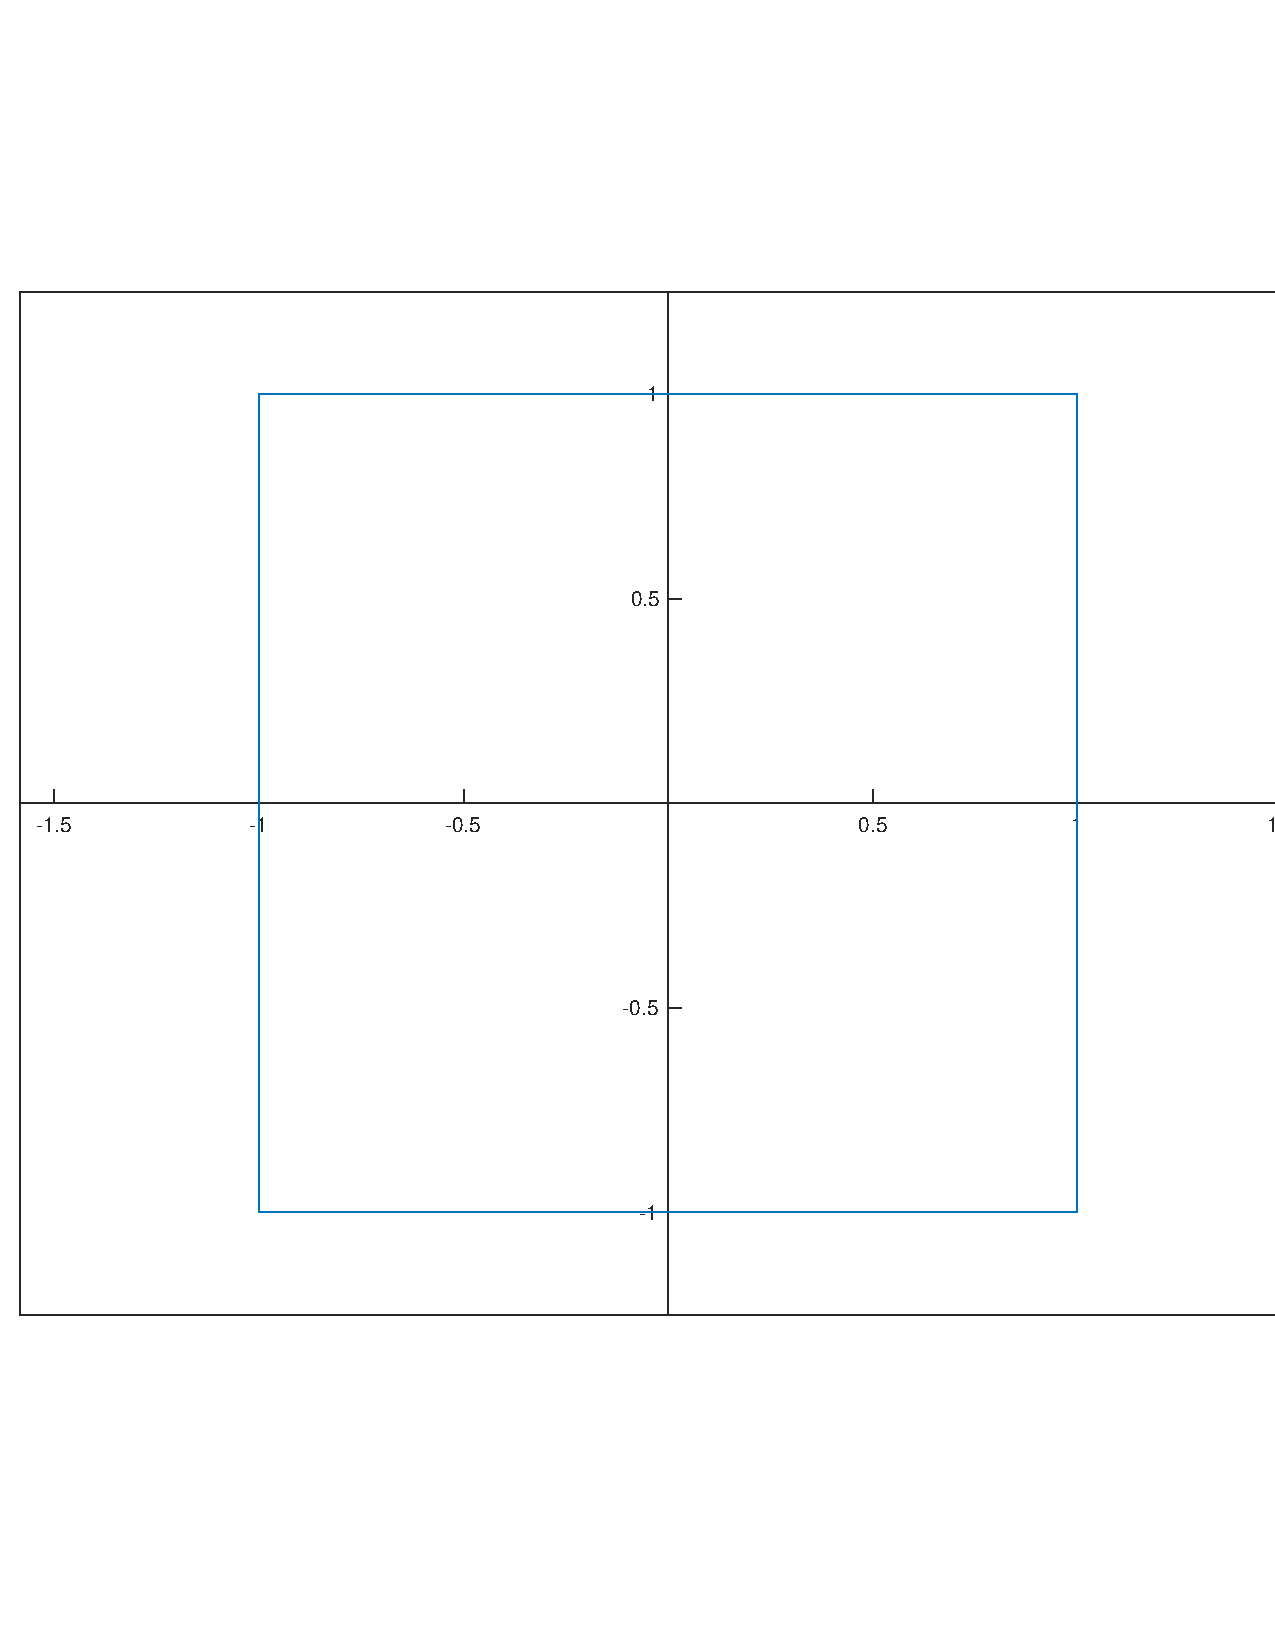
\includegraphics[scale=0.4]{unit_sphere_supnorm.pdf}
    \end{center}



\end{enumerate}

\end{document}
